\chapter{Entwurf}\label{ch:entwurf}
In den folgenden Abschnitten werden die inhaltlichen Anforderungen bezüglich der Projektziele beschrieben. Diese werden in Form von Personas und User Stories dargestellt. Dazu passend werden anschließend die grafischen Anforderungen mithilfe eines Styleguides und eines Prototyps verdeutlicht. Zuletzt werden unterschiedliche Entwicklungsumgebungen und Frameworks evaluiert, um so zu erschließen, welche sich am besten für das Projekt eignen.

\section{Inhaltliche Anforderungen}\label{inhaltliche_anforderungen}
Um de Aufteilung und Erstellung der inhaltlichen Anforderungen einfacher zu gestalten, wurden zunächst Personas entwickelt. Die Persona-Methode ist im UX-Design eine beliebte Herangehensweise, um für alle Projektbeteiligten eine gewisse Nähe zu den Nutzergruppen herzustellen.

Bei Personas handelt es sich um fiktive Personen, die als Stellvertreter für eine bestimmte Zielgruppe stehen. Sie werden mithilfe von Hintergrundinformationen einer realen Person aus der Zielgruppe entwickelt. Da TraWo ursprünglich für Nutzer von allen Altersgruppen gedacht ist und sich somit an mehrere Zielgruppen richtet, soll durch die Personas klar werden, welche Nutzer hierbei besonders im Vordergrund stehen: Eltern und Kinder.

Des Weiteren bietet das Persona-Konzept gegenüber der Arbeit mit gesichtslosen Gruppen zahlreiche Vorteile und ist somit eine passende Entscheidung für unser Team. Eines dieser Vorteile ist, wie bereits mehrmals angedeutet, die Veranschaulichung der Zielgruppen, wonach sich das Projekt richtet. Dieses Merkmal ist nicht nur einer der wichtigsten Erkennungen, sondern auch gleichzeitig eines der Ziele des Persona-Konzepts. Während des Arbeitsprozesses helfen Personas vor allem dabei, die eigentliche Zielgruppe nicht aus den Augen zu verlieren. Sie bieten nicht nur Vorteile bezüglich der Zielgruppen, sondern fördern auch gleichzeitig den kreativen Prozess im Laufe der Entwicklung. Außerdem werden im Gegensatz zu einer pauschalen Gruppe, Bedürfnisse von Personas besser an das Entwicklerteam übermittelt. (vgl. \cite{Personas})

Eine Persona besteht aus einer Art Steckbrief eines prototypischen Nutzers, welcher relevante Informationen bezüglich des Projekts enthält. Dazu gehören beispielsweise demografische Daten, Vorlieben am Produkt, Schwierigkeiten bei der Nutzung, Motivation zur Nutzung sowie Handlungskontexte bezogen auf das Produkt. In dem Fall von TraWo werden nur die für den Verlauf der Entwicklung entscheidenden Merkmale verwendet.

Wie in Abbildung \ref{fig:persona_thorsten} zu sehen ist, handelt es sich bei der ersten Persona um Thorsten. Er ist acht Jahre alt und besucht aktuell die Grundschule. In seiner Freizeit verbringt er sehr gerne Zeit am Tablet. Aus diesem Grund wünscht er sich eine Anwendung, die ihm das konventionelle Lernen mit Schulbüchern durch ein Spiel ersetzt.

Bei der nächsten Persona, die in Abbildung \ref{fig:persona_mark} zu erkennen ist, handelt es sich um Mark. Er ist 38 Jahre alt und ist momentan in der IT-Branche tätig. Er hat einen achtjährigen Sohn namens Thorsten. Aus seiner Liebe zu Computern ist es Mark besonders wichtig, seinen Sohn auch auf eine technische Art und Weise beim Lernen zu unterstützen und somit seine Bildung zu fördern. Er sucht nach einem Produkt, welches nicht nur zur Unterstützung beim Lernen dient, sondern auch die Motivation seines Sohnes erweckt.

Im Anschluss können mithilfe der zuvor entwickelten Personas Anforderungen in Form von User Stories erstellt werden.

Bei einer User Story handelt es sich um eine kurze Erläuterung einer Funktion, die sich aus den Wünschen eines Nutzers ergeben könnte. Warum wir uns für User Stories entschieden haben, liegt vor allem daran, dass sie für jeden aus dem Team leicht zu verstehen sind. Dabei ist es zu beachten, die Aufgaben so zu formulieren, dass sie auch von Beteiligten ohne technische Hintergründe verstanden werden können. Außerdem ist es so möglich, die unterschiedlichen Anforderungen in kleinere Aufgaben zu unterteilen, um so bessere Ergebnisse bis zu den regelmäßigen Meetings zu erhalten. Nach der Erstellung der User Stories werden im Team \textquote{Story Points} vergeben. Diese beschreiben die Größe und den damit entstehenden Aufwand einer User Story. Auf diese Funktion wurde in unserem Fall bewusst verzichtet, da keine große Anzahl an Anforderungen vorhanden ist. Stattdessen wurde entschieden, die Aufgaben nach Wichtigkeit zu sortieren. So war es einfacher für das Team herauszufinden, welche Aufgaben in dem Moment Vorrang haben. (vgl. \cite{UserStories})

Im Bezug auf TraWo wurde die Persona Mark zur Erstellung eines Szenarios genutzt. Dieses soll dabei helfen, einen Einblick in das vorliegende Problem zu bekommen. Aus diesem Problem wurden anschließend User Stories entwickelt, die aus der Sicht von Thorsten formuliert sind.

\textbf{Szenario:}
Mark möchte eine App für seinen Sohn, die ihm auf eine spielerische Art und Weise geografisches Allgemeinwissen beibringt.

\textbf{User Stories:}
\begin{itemize}
\item \textquote{Als Thorsten möchte ich innerhalb der App Zugriff auf ein Menü haben.}
\item \textquote{Als Thorsten möchte ich ein On-Boarding, dass mir kurz erklärt, wie die App funktioniert.}
\item \textquote{Als Thorsten möchte ich mich zwischen dem Informationsteil und dem Spielteil entscheiden können, damit ich auch ohne Benutzung der Kamera Zugriff auf die Informationen zu den Ländern habe.}
\item \textquote{Als Thorsten möchte ich im Spielteil mit meiner Tablet-Kamera die vorhandene Weltkarte erkunden. Dazu möchte ich schnell erkennen, welche Orte erkundbar sind.}
\item \textquote{Als Thorsten möchte ich das erlangte Wissen über ein freigeschaltetes Land nun prüfen. Durch das Scannen des Landes möchte ich ein Quiz starten können.}
\item \textquote{Als Thorsten möchte ich mit den Ländern in allen Kontinenten interagieren können. Durch Scannen eines Landes im Kontinent möchte ich die Möglichkeit bekommen, mich über dessen Fakten zu informieren.}
\item \textquote{Als Thorsten möchte ich, dass die Antworten der Fragen zum Teil aus dem jeweiligen Informationsteil des Landes hervorgehen. So kann ich meinen Lernfortschritt mithilfe von dem Quiz prüfen.}
\item \textquote{Als Thorsten möchte ich nach Beendigung von einem Quiz die Möglichkeit haben, von diesem zurück zur Kameraansicht zu gelangen oder Informationen zum jeweiligen Land zu erhalten.}
\item \textquote{Als Thorsten möchte ich nach Beendigung aller Quizze innerhalb meines Heimatkontinents den nächsten freischalten können, damit ich motiviert bleibe.}
\end{itemize}

\section{Grafische Anforderungen}

\subsection{Styleguide}\label{styleguide}
Bei einem Styleguide handelt es sich um ein Dokument, das als Leitfaden für alle grafischen Elemente und Merkmale einer Anwendung dient. Er gibt an, auf welche Gestaltungsrichtlinien das Team während der Entwicklung Wert legen sollte, um so zukünftige Probleme zu vermeiden. Denn je später solche Fehler entdeckt werden, desto höher ist der Aufwand der Änderung. Es kann nämlich dazu kommen, dass die Änderung dadurch nicht nur an einem Element, sondern an dem ganzen Projekt durchgeführt werden muss. Aus diesem Grund sollte ein Styleguide im Idealfall mit Beginn des Projekts existieren. Da dieser jedoch parallel zum Projekt läuft, empfiehlt es sich, ihn kontinuierlich weiterzuentwickeln und zu optimieren.

Styleguides können beispielsweise grafische Inhalte und Informationen in Form von Logos, Schriftvorgaben, Farbvorgaben oder Briefbögen beinhalten. Da jedoch jeder Anwendungsfall unterschiedliche Verwendungszwecke oder Anforderungen besitzt, können die Inhalte variieren. Aus diesem Grund ist es wichtig, im Voraus zu klären, welche Punkte darin auf jeden Fall behandelt werden müssen. Grundsätzlich sollten diese Inhalte möglichst einfach zu verstehen sein. Auf komplizierte Formulierungen wird verzichtet, um so ein gut strukturiertes Dokument schaffen zu können. (vgl. \cite{Styleguide})

\begin{figure} [h]
\centering
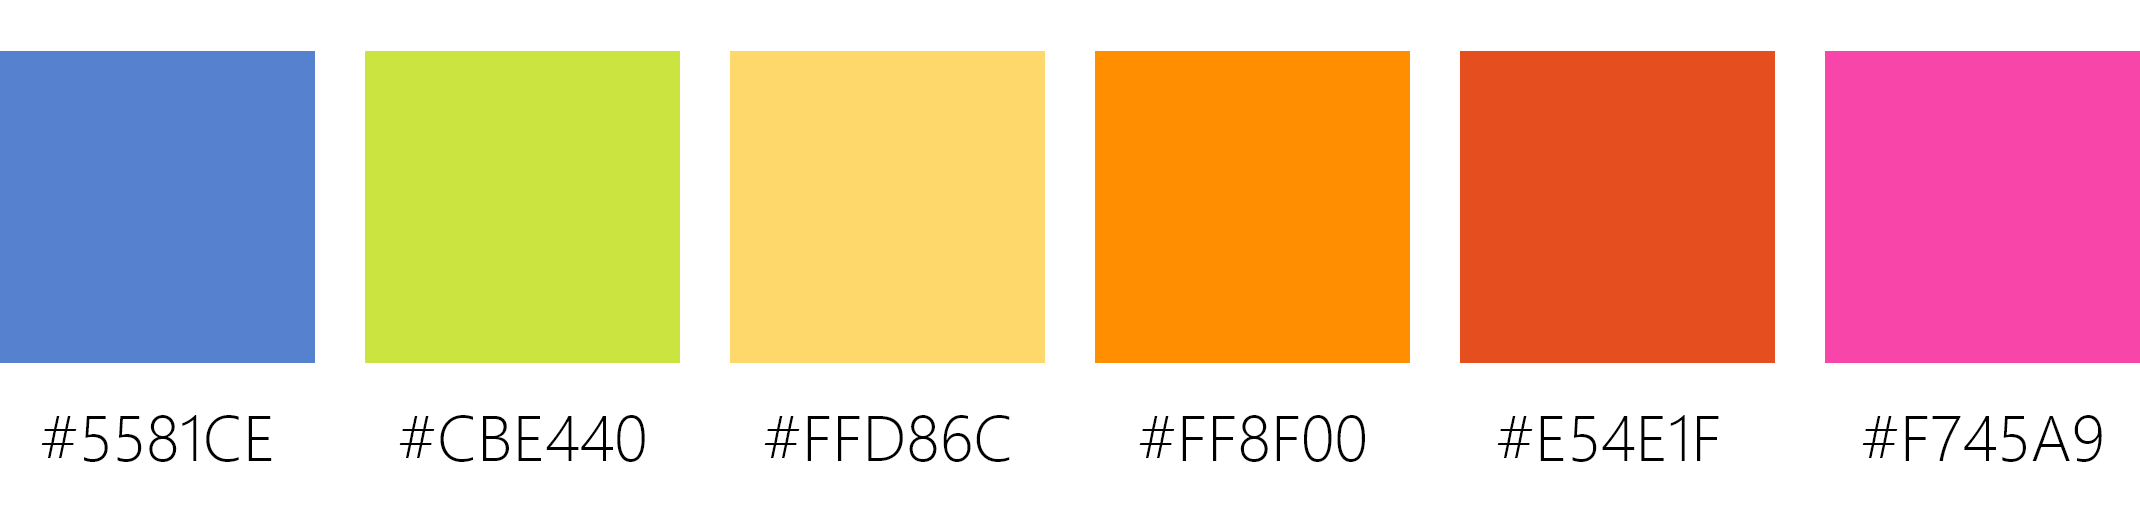
\includegraphics[width=12cm]{Farben.PNG}
\caption{Verwendete Farbpalette}
\label{fig:farben}
\end{figure}

In unserem Fall wurde der Styleguide hauptsächlich zur Dokumentation der Schrift- und Farbvorgaben genutzt. Da sich TraWo in erster Linie an Kinder richtet, war es besonders wichtig, das Farbschema bunt und ansprechend zu halten. Abbildung \ref{fig:farben} zeigt das gewählte Farbschema.

\begin{figure} [h]
\centering
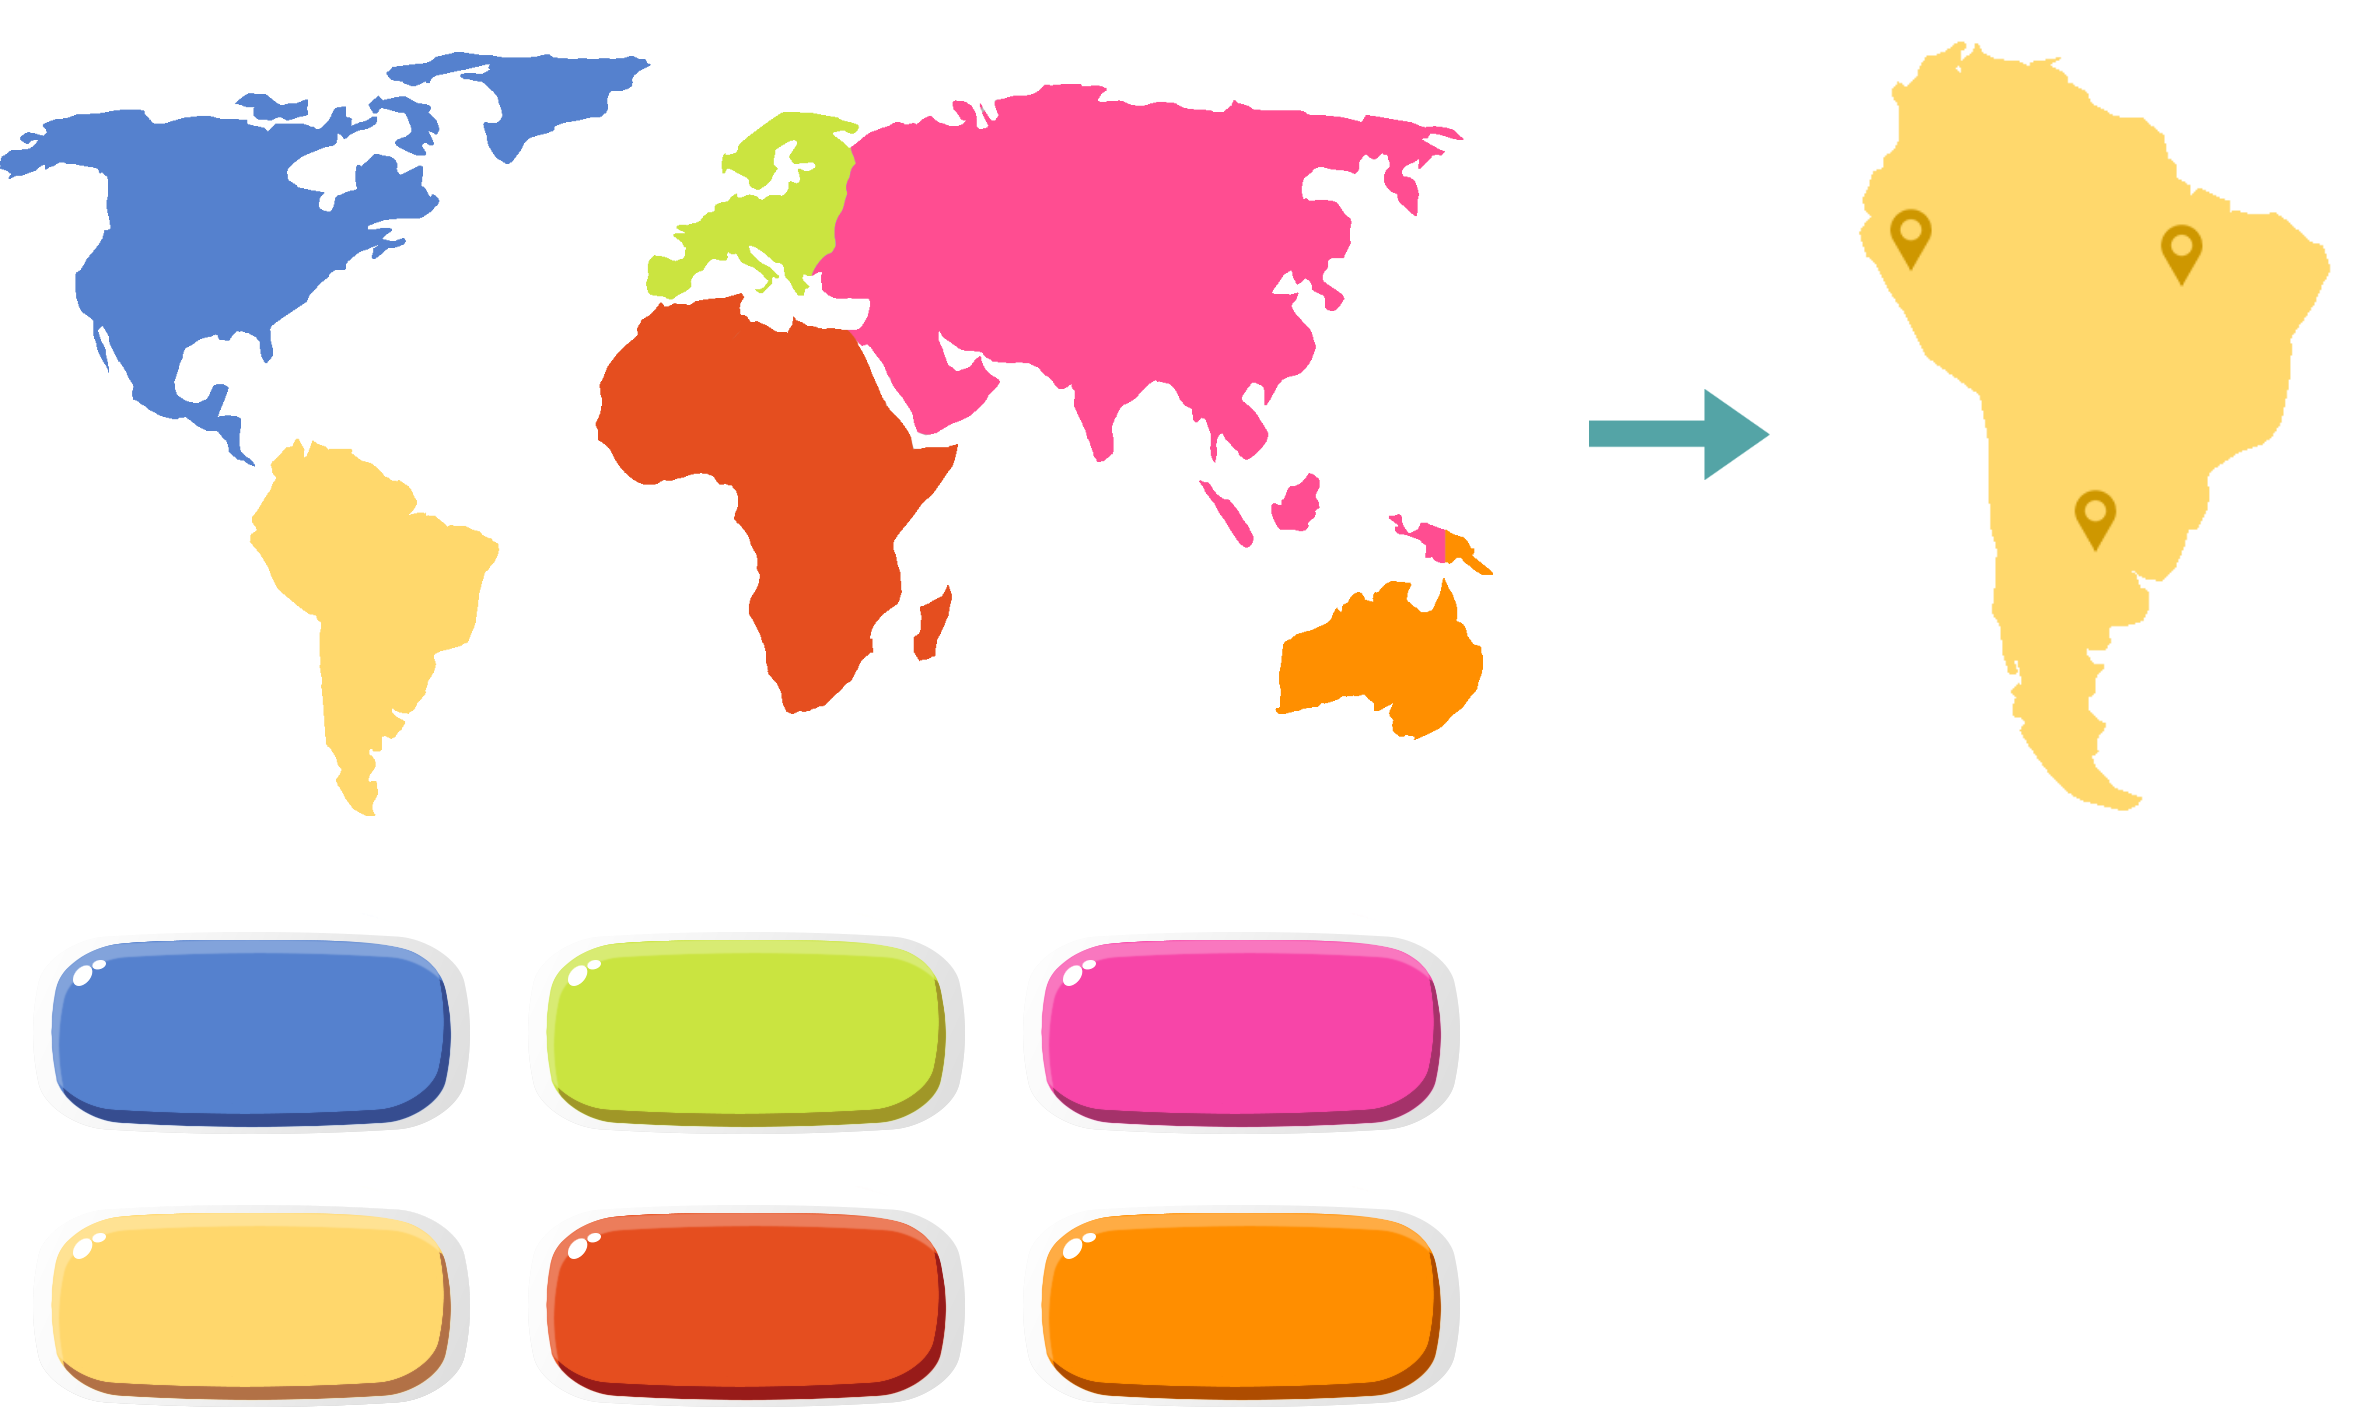
\includegraphics[width=13cm]{Map.PNG}
\caption{Landkarte und Buttons in dem genannten Farbschema}
\label{fig:map}
\end{figure}

Wie in Abbildung \ref{fig:map} zu sehen, ist wurde die oben genannte Farbpalette auf die Landkarte und die Buttons übertragen. Diese finden im Verlauf der App immer wieder an Bedeutung. Die Farben sollen vor allem zum Verständnis der Landkarte dienen und durch die Buttons zeigen, wo sich welcher Kontinent befindet. Nach der Wahl eines Kontinents soll durch Standortsymbole gekennzeichnet werden, welche Länder zur Auswahl stehen.

\subsection{Prototyp}\label{prototyp}
Ein weiterer wichtiger Schritt, der nach einem Styleguide folgt, ist die Entwicklung eines Prototyps. Abbildung \ref{fig:flowchart} zeigt, dass dieser in unserem Fall in Form eines Flowchart-Modells dargestellt wurde.

\begin{figure} [h]
\centering
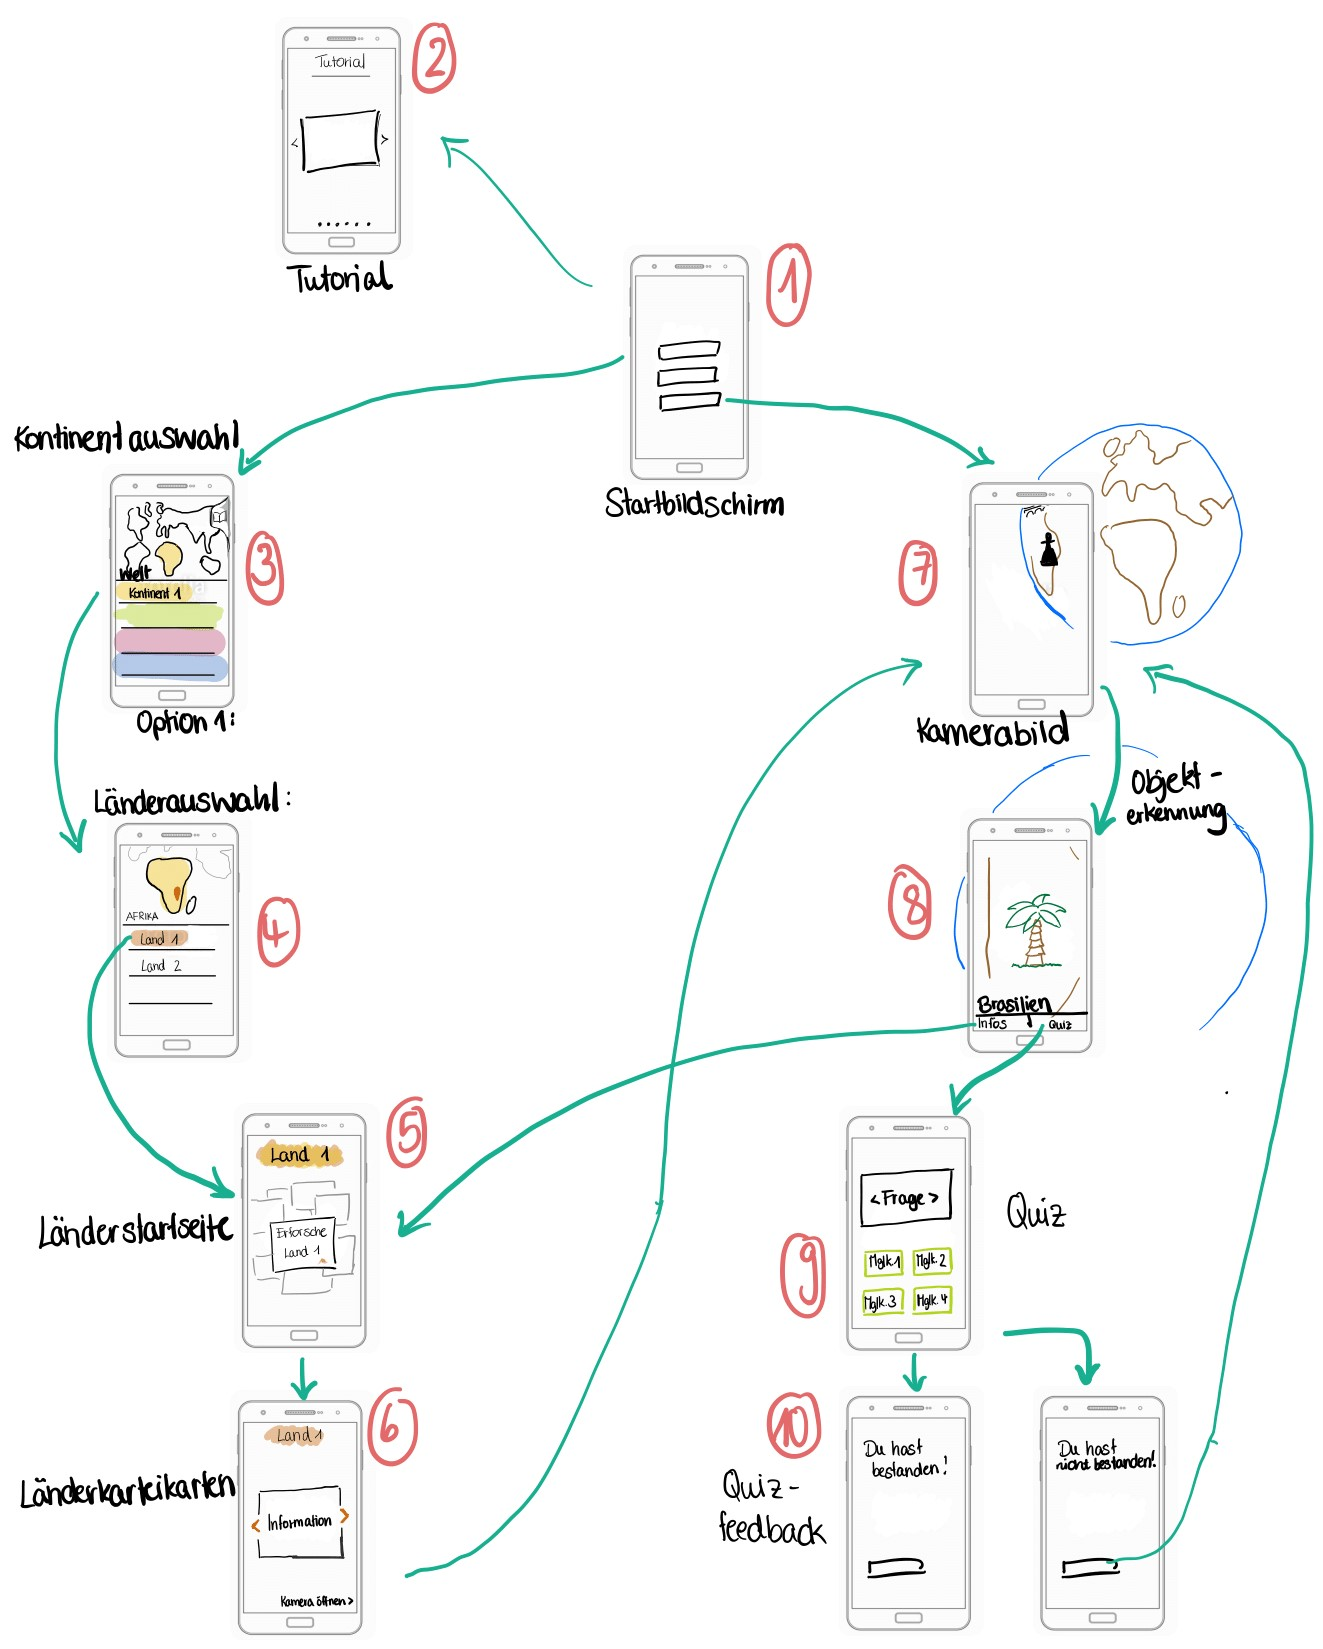
\includegraphics[width=13.5cm]{flowchart.JPG}
\caption{Prototyp in Form eines Flowchart-Modells}
\label{fig:flowchart}
\end{figure}

Ein Prototyp ist ein Beispiel, das als Grundlage für eine zukünftige Oberfläche dient. Es bietet die Möglichkeit, die Funktionalität des vorhandenen Designs oder Konzepts vor der Entwicklung zu testen. Somit kann vor allem Zeit gespart werden, falls Änderungswünsche während des Tests auffallen. Außerdem ist es so möglich wertvolle Rückmeldung von anderen Teammitgliedern zu erhalten, bevor das eigentliche Projekt gestartet wird. Ein einfacher Prototyp bietet außerdem mehr Freiraum bei der Entwicklung und vermeidet, dass man an kleinen Details hängen bleibt. In unserem Fall wurde der Prototyp hauptsächlich dazu genutzt einen groben Überblick für das Team zu schaffen. So hat man bereits eine Vorstellung, wie das fertige Produkt aussehen könnte und kann im Anschluss ohne Probleme mit der Entwicklung beginnen.

Der Prototyp wurde mithilfe der Anforderungen in den User Stories aus Abschnitt \ref{inhaltliche_anforderungen} erstellt. Zur Darstellung wurde sich wie bereits erwähnt für ein Flowchart-Modell entschieden. Bei einem Flowchart handelt es sich um eine grafische Darstellung des Prozesses, der die Schritte und Funktionen der einzelnen Fenster beschreibt.

Wie man in Abbildung \ref{fig:flowchart} erkennen kann, beginnt die Anwendung mit einem klassischen Hauptmenü. Von dem Menü aus ist es möglich, mit einem Tutorial zu beginnen. Dieses beschreibt in kurzen Sätzen die Funktionalität von TraWo. Ansonsten teilt sich die Anwendung in zwei Teilbereiche auf. Zum einen gelangt man in den Informationsteil, welcher von den Punkten drei bis sechs zu sehen ist. Der Nutzer entscheidet sich zunächst für einen Kontinent und wird anschließend zur Länderauswahl weitergeleitet. Von da aus gelangt er zu den Lernkarten, die die Informationen zu dem gewählten Land wiedergeben. Der zweite Teilbereich, der von den Punkten sieben bis zehn zu sehen ist, beschreibt den Augmented Reality Teil. Von hier aus ist es möglich, zum Quiz zu gelangen. Anschließend führt dieses den Nutzer je nach Ergebnis zum jeweiligen Feedback Fenster.

\section{Architekturentscheidung} \label{architekturentscheidung}
Um die inhaltlichen und grafischen Anforderungen von TraWo realisieren zu können, mussten wir uns auf eine Entwicklungsumgebung, sowie genutzte Frameworks zur Nutzung von Augmented Reality Elementen einigen. Der folgende Abschnitt beschreibt das durchgeführte Evaluationsverfahren zur Auswahl einer IDE und benötigten Tools.
\subsection{Entwicklungsumgebung}\label{entwicklungsumgebung}
Für die Entwicklungsumgebung haben sich von Anfang an zwei Favoriten herauskristallisiert. Die Wahl bestand zwischen der Gaming-Engine \textquote{Unity} und der \textquote{Android Studio} IDE. Im Folgenden werden Vor- und Nachteile der beiden Plattformen aufgelistet.

Bei der Entwicklung einer Android Applikation liegt, bei erster Betrachtung, die Wahl der Entwicklungsumgebung Android Studio nahe. Die Umgebung ist speziell für die klassische mobile Appentwicklung prädestiniert und soll den Entwickler dabei unterstützen, eine native Android-Applikation zu erstellen. Grundsätzlich bietet Android Studio auch einige Schnittstellen zu Augmented Reality Frameworks, wie beispielsweise \textquote{ARCore} an. Da die meisten Teammitglieder wenig bis keine Erfahrung mit der Umgebung haben, wäre es zudem ein aufschlussreiches Erlebnis, diese IDE näher kennenzulernen.

Ein größeres Problem hingegen, entsteht durch das Fehlen einer integrierten 3D-Engine in Android Studio. Dadurch ist es nicht ohne Weiteres möglich, 3D-Objekte auf dem Handybildschirm zu rendern, was jedoch eine der Hauptanforderungen für die Lernapplikation darstellt. Diese Möglichkeit wäre dennoch gegeben, wenn man externe Tools wie \textquote{OpenGL} verwendet. Aus Recherchen zeigt sich jedoch, dass der Umgang damit nicht besonders einsteigerfreundlich und somit mit hohem Aufwand verbunden ist.

Der Gegenkandidat Unity ist zunächst eher aus der Videospielentwicklung bekannt. Bereits im dritten Semester durften wir alle im Fach \textquote{Software Engineering} ein Spiel mit der Engine programmieren. Damit hätte jeder aus der Gruppe zumindest eine gewisse Grunderfahrung mit der Umgebung. Auch wenn es sich zunächst kontraintuitiv anhört, Unity für eine Android-App zu benutzen, bei der es sich nicht um einen 2D-Platformer handelt, so gibt es einige Punkte, die überzeugender Weise dafür sprechen.

Grundsätzlich stellt Unity die einfache Möglichkeit bereit, die geschriebenen Skripte in eine .apk-Datei über ein integriertes Software Development Kit (SDK) umzuwandeln. Das ermöglicht uns, die für uns bequeme Programmiersprache C\# zu nutzen und gleichzeitig problemlos eine auf dem Smartphone laufende Anwendung zu erzeugen. Gute Schnittstellen zu diversen AR-Frameworks wie \textquote{AR-Core} oder \textquote{Vuforia} sind vorhanden und lassen sich leicht konfigurieren. Unitys interne 3D-Enginge ermöglicht außerdem eine aufwandslose Anzeige von Augmented Reality Inhalten. Aus der eigenen Erfahrung zeigt sich allerdings, das Unity nicht vorwiegend für eine gestaltungsorientierte Entwicklung geeignet ist. Eventuell müsste man beim Erstellen der GUI für TraWo auf Kompromisse eingehen.

Das Team war zunächst eher dazu geneigt, mit Android Studio zu arbeiten. Auch wenn auf dem Papier Unity einem Entwickler mit der internen 3D-Engine scheinbar deutlich mehr abzunehmen scheint, hat sich für uns die Arbeit mit dem nativen Appentwickler Studio doch aufregender angehört. Bevor wir aber eine Entscheidung fällen konnte, mussten wir erst überprüfen, ob es ein favorisiertes AR-Framework gibt, welches vielleicht in Kombination mit einer der beiden IDEs als besonders erfolgreich gilt.

Alternativen wie Xamarin oder Flutter kamen für unsere Entwicklung hauptsächlich aufgrund von mangelnden Schnittstellen zu externen Frameworks nicht in Frage.
\subsection{Mustererkennung}
Das Ziel des AR-Frameworks ist es, mit Hilfe der Kamera des genutzen Smartphones, ein vorher definiertes Muster zu erkennen und eine darauf abgestimmte Reaktion abzugeben. Neben allgemeinen Erfahrungsberichten aus diversen Foren, auf die wir uns berufen haben, wurden von uns vier Kriterien aufgestellt, anhand derer wir verschiedene Framewoks miteinander verglichen haben:
\begin{itemize}
\item Tracking Stabilität
\item Dokumentation
\item Aktiver Community Support
\item Markerless Tracking Option
\end{itemize}
Die Tracking Stabilität ist ein allgemeines Qualitätssiegel dafür, wie gut die Mustererkennung des Systems funktioniert. Anzeichen dafür sind unter anderem, wie gut die Umweltbedingungen wie beispielsweise die Beleuchtung sein müssen, damit das Muster erkannt wird. Sollte diese Bewertung unterdurchschnittlich schlecht sein, käme das Framework nicht in Frage.
Um die Einarbeitung möglichst angenehm gestalten zu können, sollte das Framework über eine verständliche Dokumentation verfügen.
Falls im Laufe der Entwicklung ungeklärte Fragen auftauchen sollten, sind aktive Nutzerforen oft sogar von größerem Vorteil als die offizielle Dokumentation selbst. 

Es gibt grundsätzlich zwei Arten von Mustererkennung: Die \textquote{markerbasierte} und die \textquote{markerlose}. Wie bereits in Abschnitt \ref{projektziel} angedeutet, ist es unser Ziel, festgelegte Marker zu nutzen. Die Funktionalität dahinter wird nachher in Abschnitt \ref{einbindung_mustererkennung} näher beschrieben. Dennoch wollten wir uns die alternative \textquote{markerlose} Musterkennung, welche sich mehr auf einen Kontext in der Umgebung als ein bestimmtes Muster konzentriert, für eine eventuelle Änderung unserer Herangehensweise offen lassen.

{
\centering
\begin{tabular}{|c|c|c|c|c|c|}  
    \cline{2-6}
    \multicolumn{1}{c|}{} & Ar-Toolkit & Kudan SDK & MaxStAR & Wikitude SDK & Vuforia  \\
    \hline
    Tracing Stabilität & \xmark & \xmark & \cmark & \cmark & \cmark \\
    \hline
    Dokumentation & \xmark & \cmark & \xmark & \xmark & \cmark \\
    \hline
    Community Support & \xmark & \xmark & \xmark & \xmark & \cmark \\
    \hline
    Markerless Tracking & \cmark & \cmark & \cmark & \cmark & \xmark \\
    \hline
\end{tabular}
}

Nach diesen Kriterien haben wir nach verschiedenen Frameworks recherchiert, unter anderem \textquote{AR-Toolkit}, \textquote{Kudan SDK}, \textquote{Wikitude}, \textquote{MaxStAR} sowie die vorher bereits erwähnten \textquote{Vuforia} und \textquote{ARCore}. Die meisten kamen jedoch aufgrund von schlechter Bewertung in der Tracking Stabilität oder einer mangelnden Anbindung zu unseren Entwicklungsumgebungen bereits nicht infrage. Ausschlaggebend bei der Recherche war letzten Endes, wie gut die Erfahrungswerte für die jeweilige Schnittstelle ausfielen. Die scheinbar beste Kombination schien aus Unity und Vuforia zu bestehen. Somit stand unsere Entscheidung fest.

\subsection{Datenhaltung und -bereitstellung}\label{datenhaltung und -bereitstellung}
Eines der großen Ziele für das Projekt ist die möglichst generische Haltung der Softwarestruktur, um leichte Ausbaufähigkeit sicherzustellen und die eventuelle Übertragung auf alternative Anwendungsfälle zu ermöglichen. Aus diesem Grund sollten appspezifische Inhalte nicht festcodiert, sondern nach Möglichkeit extern gelagert werden. Eine separate Datenbank soll dafür die Lösung bieten.

Neben einer strukturierteren Systemarchitektur, hätte die Nutzung einer Datenbank zugleich einen weiteren Vorteil: Man hat nun die Möglichkeit, Daten über die Laufzeit der Anwendung hinaus abzuspeichern. Das bedeutet, dass Informationen nach dem Schließen der App weiterhin erhalten bleiben. Somit haben wir eine Perspektive auf das Sichern von Spielfortschritt, welche vorher nicht gegeben war.

Die Verwendung einer Datenbank zur Datenhaltung und -bereitstellung stand also außer Frage. Es galt nun zu klären, wie genau sie erstellt und genutzt werden soll.

Um möglichst ressourcensparend arbeiten zu können, wurde sich schnell auf die Programmbibliothek \textquote{SQLite} zur Erstellung und Verwaltung geeinigt. Ihr Hauptvorteil ist ihr minimalistischer Aufbau. Als eines der kompaktesten Datenbanksysteme, besitzt SQLite zwar nur eine beschränkte Funktionalität für das Arbeiten mit Datenbanken, ist dafür aber für die Datenbankverwaltung vollkommen unabhängig von weiterer Software. So ist zum Beispiel, im Gegensatz zu komplexeren Bibliotheken, wie \textquote{Microsoft SQL Server}, keine weitere Serveranbindung nötig. Außerdem ist zu Unity und vielen anderen Entwicklungsumgebungen eine passende Schnittstelle vorhanden.

Die frei verfügbare Software \textquote{DB Browser for SQLite} eignet sich angemessen als graphische Benutzeroberfläche für die Arbeit direkt an der Datenbank. So lassen sich damit ganze Querys direkt ausführen, oder über Shortcuts beispielsweise Tabellen einfach erzeugen.

Die Tatsachen, dass sich SQlite denkbar einfach in die Entwicklung einbinden lässt und der geringe Speicherverbrauch des Datenbanksystems, machen die Programmbibliothek zu einem beliebten Kandidaten für die mobile Appentwicklung. Die abgeschwächte Funktionalität im Vergleich zu gewohntem SQL, sollte für uns kein Hinderungsfaktor sein, da wir davon ausgingen, keine sonderlich komplexe Datenbankstruktur aufzubauen. Für den in diesem Kontext geringen Tabellenumfang, schien es das optimale System zu sein. 

Somit standen alle zu nutzenden Technologien für das Projekt fest und es konnte mit der Realisierung angefangen werden. Bevor die eigentliche Umsetzung beschrieben wird, folgt im kommenden Abschnitt eine genau Erläuterung der Funktionsweise einiger Komponenten für eine bessere Übersicht des Projektumfangs und eines allgemeinen Verständnisses für die Arbeitsweise der entstandenen Applikation.